\begin{center}
	
	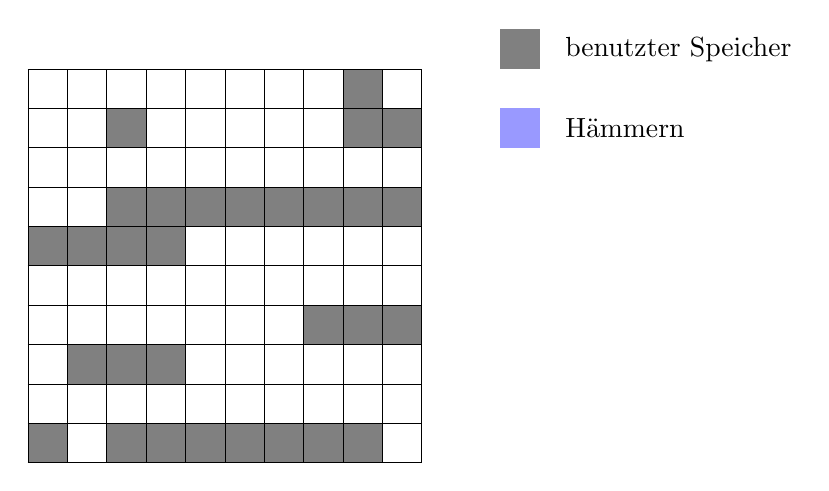
\begin{tikzpicture}
	
	\draw[step=0.5cm,very thin] (0,0) grid (5,5);
	
	% \draw[pattern=north west lines, pattern color=red] (0,0) rectangle (5,5);
	
	% Used space
	\fill[gray] (0,0) rectangle (0.5,0.5);
	\fill[gray] (1,4) rectangle (1.5,4.5);
	\fill[gray] (1,3) rectangle (5,3.5);
	\fill[gray] (0,2.5) rectangle (2,3);
	\fill[gray] (1,0) rectangle (4.5,0.5);
	\fill[gray] (0.5,1) rectangle (2,1.5);
	\fill[gray] (4,4.5) rectangle (4.5,5);
	\fill[gray] (4,4) rectangle (5,4.5);
	\fill[gray, opacity=1] (3.5,1.5) rectangle (5,2);
	
	% Bitflip
	% \draw[red!40,thin] (3,2) -- (3.5,2) -- (3.5,2.5) -- (3,2.5) -- (3,2);
	% \fill[red!40] (3,2) rectangle (3.5,2.5);

	% hammer
	% \fill[blue!40] (2.5,2) rectangle (3,2.5);
	
	% Legende
	\filldraw[gray, label=0:end] (6,5) rectangle (6.5,5.5);
	\node[right] at (6.7,5.25) {benutzter Speicher};
	
	\draw[blue!40,thin] (6,4) -- (6.5,4) -- (6.5,4.5) -- (6,4.5) -- (6,4);
	\fill[blue!40] (6,4) rectangle (6.5,4.5);
	\node[right] at (6.7,4.25) {Hämmern};
	
	% \draw[red!40,thin] (6,3) -- (6.5,3) -- (6.5,3.5) -- (6,3.5) -- (6,3);
	% \fill[red!40] (6,3) rectangle (6.5,3.5);
	% \node[right] at (6.7,3.25) {Bitflip};
	
	% \draw[thin] (6.1,2.1) -- (6.4,2.4);
	% \draw[thin] (6.4,2.1) -- (6.1,2.4);
	% \node[right] at (6.7,2.25) {geladene Binary};
	
	\draw[step=0.5cm,very thin] (0,0) grid (5,5);
	
	\end{tikzpicture}
	
\end{center}